% !TeX root = ../main.tex
\chapter{Crawler Design and Mechanical Validation}
\label{chap:crawler}
\label{chap:methods}
% Retain chap:methods for existing links from Chapters 1, 3, and 5.
% Other chapter files are intentionally unchanged in this revision.
\begingroup
\setlength{\emergencystretch}{3em}
\clubpenalty=10000
\widowpenalty=10000
\newcommand{\mechanicalplaceholder}[3]{%
\begin{figure}[htbp]
\centering
\fbox{\begin{minipage}[c][32mm][c]{0.88\textwidth}
\centering\small\singlespacing\textbf{IMAGE PLACEHOLDER}\par\medskip #1
\end{minipage}}
\caption{#2}\label{#3}
\end{figure}}

This chapter documents the existing crawler and defines the mechanical checks needed to support its vacuum equipment during deployment and operation. The calculations are verification of the assembled design; they are not presented as calculations completed before construction. The scope covers drive demand, equipment integration, the retrieval load path, and measured pulling capability. Vacuum generation and compressed-air characterization remain in Chapter~\ref{chap:vacuum}.

\textbf{Verification status.} The available records do not include a completed mass budget, verified motor performance curves, attachment load limits, or mechanical test data. Numerical conclusions and simulation results therefore remain pending. The figures marked as placeholders identify the motor photographs, current computer-aided design (CAD) views, and analysis outputs required to complete the chapter.

\section{Design Requirements}
\label{sec:mechanical-requirements}
The complete crawler must pass through the confirmed 12-inch-diameter opening, equivalent to 304.8~mm. The deployed assembly includes the wheels, vacuum units, collection hardware, electronics, fittings, and connected services. Width and height checked separately against the opening are insufficient; the assembly must fit within its circular cross section throughout the intended insertion sequence, with an allowance for handling and manufacturing variation.

The frame must support the operating equipment and an explicitly defined maximum debris mass in the collection bag. This full-bag condition is a design assumption until its mass and location are specified. Bag volume alone does not define payload. The 32-inch wall-to-wall annulus spacing and 0.75-inch protective-pipe outside diameter remain the confirmed project requirements. Local floor curvature and the installed pipe supports must be represented when assessing clearance; pipe diameter is not automatically the obstacle's exposed height.

For this chapter, the author specifies a 100-ft (30.48~m) compressed-air hose, a power/Ethernet tether, and a rear attachment. The tether's length, mass distribution, and support arrangement still require confirmation. The crawler must start, travel, turn, and cross the representative pipes with these services connected. Deployment and retrieval must transfer the applicable loads through the designated attachment into the frame. Whether the same attachment is approved for lifting, horizontal recovery, and angled recovery must be established before assigning its working load.

\section{Motor Selection and Torque Calculations}
\label{sec:motor-verification}
Wang et al. organize their chassis power calculation around rolling resistance, slope resistance, traction force, and travel power \citep{wang2024CrawlerChassis}. This sequence is useful here, but their agricultural-track coefficients, slope, power values, and engine margin are not transferred to the vacuum crawler. The following balance adds the external service-line forces and uses consistent SI units: mass in kilograms, force in newtons, torque in newton-metres, and power in watts.

\subsection{Mass Budget and Payload}
Let $m_0$ be the empty operating assembly mass and $m_d$ the assumed maximum debris mass. The loaded crawler mass is
\begin{equation}
 m=m_0+m_d, \qquad
 m_0=\sum_k m_k.
 \label{eq:crawler-mass}
\end{equation}
The component sum is an alternative to, and a check on, a measured assembly mass. Components already included in a weighed assembly must not be added again. Table~\ref{tab:crawler-mass-budget} identifies the contributions. Only hose or cable segments carried onboard belong in $m_0$; the externally routed bundle is treated separately.

\begin{table}[htbp]
\centering
\caption{Mass budget to be completed for the tested crawler configuration.}
\label{tab:crawler-mass-budget}
\begingroup\small\singlespacing
\renewcommand{\arraystretch}{1.2}
\begin{tabularx}{\textwidth}{@{}p{0.39\textwidth}p{0.15\textwidth}X@{}}
\toprule
Contribution & Mass (kg) & Required identification \\
\midrule
Frame and structural mounts & Pending & Material, revision, included brackets \\
Motors and transmissions & Pending & Quantity, model, included gearheads \\
Wheels, hubs, and tires & Pending & Quantity and installed tire configuration \\
Electronics and enclosure & Pending & Complete operating contents \\
Onboard Venturi units & Pending & One- or two-unit configuration \\
Empty bag and collection hardware & Pending & Bag, cage, inlet, and fittings \\
Other onboard fittings/services & Pending & Items not included above \\
Maximum debris payload $m_d$ & Assumed; unset & Material, mass, and bag location \\
\bottomrule
\end{tabularx}
\endgroup
\end{table}

Record the empty assembly mass on a calibrated scale, reconcile it with the component inventory, and add only the selected debris payload. The loaded center of mass follows $\boldsymbol r_G=\sum_k m_k\boldsymbol r_k/m$, including the debris contribution. The representative full-bag location must follow the actual bag support; a mass placed arbitrarily on top of the crawler does not reproduce that loading.

\subsection{Hose and Tether Resistance}
The baseline route is a straight, level corridor without bends, edge contact, or snagging. For each line $j$, distinguish floor-supported length $L_{f,j}$, suspended length $L_{s,j}$, and length supported externally $L_{e,j}$. These portions account for the external line length. For the air hose, their sum is 30.48~m less any segment already included onboard. The partition may change as the crawler moves and must be recorded at the evaluated position.

For a freely sliding floor-supported segment, a preliminary resistance model is
\begin{equation}
 D_f=\sum_j \mu_j\lambda_j gL_{f,j},
 \label{eq:line-drag}
\end{equation}
where $\lambda_j$ is mass per unit length, $\mu_j$ is the effective sliding coefficient, and $g$ is gravitational acceleration. This applies the sliding-friction relation to the supported line weight \citep{openstaxFriction}. Starting resistance requires its own measurement or coefficient. Binding between bundled lines, connector drag, and changes in pressure or line shape should be represented by measuring the actual bundle rather than assuming this model is exact.

Suspended portions transmit tension according to their routing and external supports. Their full weight is not automatically carried by the crawler. Let the resultant line force at the rear attachment be $(-D,H)$ in the forward and upward directions, respectively. $D$ is the opposing longitudinal component, including floor drag and any suspended-line contribution; $H$ is signed and may act upward or downward. Until the routing and support reactions are known, these components remain parameters. If the endpoint force is measured directly, do not add Equation~\ref{eq:line-drag} to it a second time. Bends and edge contact are excluded from this baseline and need separate evaluation if present in deployment.

\subsection{Driving Force, Wheel Loading, and Motor Demand}
Figure~\ref{fig:crawler-force-diagram} defines the level-floor force model. For straight motion on a local slope $\alpha$, taken as positive uphill, a first estimate is
\begin{align}
 N &= mg\cos\alpha-H, \\
 F_{\mathrm{req}} &= C_{rr}N+D+mg\sin\alpha+ma.
 \label{eq:crawler-driving-force}
\end{align}
Here $N$ is total wheel normal load, $C_{rr}$ is an effective dimensionless rolling-resistance coefficient, and $a$ is forward acceleration. On a slope, $D$ and $H$ are resolved parallel and normal to the surface. The baseline uses $\alpha=0$; a nonzero slope is included only when its geometry is specified. The force balance neglects aerodynamic resistance at the intended low speed and treats wheel/rotor rotational inertia separately. $C_{rr}$ must describe the installed tires and floor, not agricultural tracks.

\begin{figure}[htbp]
\centering
\resizebox{0.96\textwidth}{!}{%
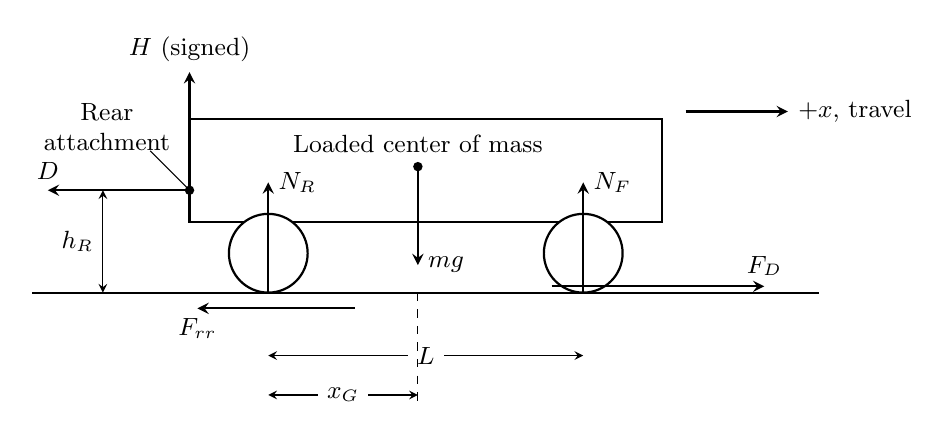
\begin{tikzpicture}[>=stealth,force/.style={->,thick},font=\small]
\draw[thick] (-2,0)--(8,0);
\draw[thick] (0,0.9) rectangle (6,2.2);
\draw[thick,fill=white] (1,0.5) circle (0.5);
\draw[thick,fill=white] (5,0.5) circle (0.5);
\fill (2.9,1.6) circle (0.06);
\node[above] at (2.9,1.65) {Loaded center of mass};
\draw[force] (2.9,1.6)--(2.9,0.35) node[right] {$mg$};
\fill (0,1.3) circle (0.06);
\draw[force] (0,1.3)--(-1.8,1.3) node[above] {$D$};
\draw[force] (0,1.3)--(0,2.8) node[above] {$H$ (signed)};
\node[align=center] at (-1.05,2.1) {Rear\\attachment};
\draw (-0.5,1.8)--(0,1.3);
\draw[force] (1,0)--(1,1.4) node[right] {$N_R$};
\draw[force] (5,0)--(5,1.4) node[right] {$N_F$};
\draw[force] (4.6,0.08)--(7.3,0.08) node[above] {$F_D$};
\draw[force] (2.1,-0.2)--(0.1,-0.2) node[below] {$F_{rr}$};
\draw[<->] (1,-0.8)--(5,-0.8) node[midway,fill=white] {$L$};
\draw[dashed] (2.9,0)--(2.9,-1.4);
\draw[<->] (1,-1.3)--(2.9,-1.3) node[midway,fill=white] {$x_G$};
\draw[<->] (-1.1,0)--(-1.1,1.3) node[midway,left] {$h_R$};
\draw[force] (6.3,2.3)--(7.6,2.3) node[right] {$+x$, travel};
\end{tikzpicture}}
\caption[Level-floor crawler force model]{Level-floor force model, not a dimensioned drawing. $N_R$ and $N_F$ are rear and front axle load sums; $F_D$ is total forward wheel force and $F_{rr}$ is rolling resistance. The rear attachment coordinate $x_R$ is measured from the rear contact line and may be negative.}
\label{fig:crawler-force-diagram}
\end{figure}

The rear force also changes wheel loading. For level, quasi-static travel, neglecting small rolling-resistance moments, moment and vertical-force equilibrium give
\begin{equation}
 N_F=\frac{mgx_G-x_RH-h_RD}{L}, \qquad
 N_R=mg-H-N_F.
 \label{eq:crawler-axle-loads}
\end{equation}
$L$ is the distance between axle contact lines, $x_G$ is the loaded center-of-mass distance ahead of the rear contact line, and $(x_R,h_R)$ locates the rear attachment. This is a sagittal-plane equilibrium model, not a four-wheel load solution. Negative axle reactions indicate loss of the assumed contact state. Unequal wheel elevations and lateral loading require the actual support geometry; contact forces and external moments govern stability \citep{papadopoulos1996Stability}. Acceleration-induced load transfer is outside this quasi-static relation.

For common loaded wheel radius $r$, total wheel torque is estimated as
\begin{equation}
 \tau_{w,\mathrm{tot}}=rF_{\mathrm{req}}+\tau_{\mathrm{rot}},
 \qquad P_{\mathrm{travel}}=F_{\mathrm{req}}v,
 \label{eq:wheel-torque-demand}
\end{equation}
where $v$ is travel speed and $\tau_{\mathrm{rot}}$ accounts for acceleration of rotating components. For steady travel it is zero; if startup is evaluated, obtain it from verified inertias or identify its omission as a model limitation. Power alone cannot assess starting torque because $v=0$ at rest.

Let $\gamma_i$ be motor $i$'s share of wheel-torque demand, with $\sum_i\gamma_i=1$. With speed reduction $G_i=\omega_{m,i}/\omega_{w,i}$ and transmission efficiency $\eta_i$,
\begin{equation}
 \tau_{m,i,\mathrm{req}}=\frac{\gamma_i\tau_{w,\mathrm{tot}}}{G_i\eta_i},
 \qquad \omega_{m,i}=G_i\frac{v}{r}.
 \label{eq:motor-demand}
\end{equation}
The speed relation assumes negligible longitudinal slip. Four wheels and left-right differential control do not establish the number of motors or mechanical couplings. Equal sharing, $\gamma_i=1/n_m$, is only a preliminary assumption for $n_m$ identical equally loaded drives. The installed arrangement and unequal-load cases must be recorded before numerical evaluation. If a rating is already given at the gearmotor output shaft, compare at that shaft without applying its internal gearbox ratio again.

\subsection{Available Torque and Separate Operating Cases}
Compare the required torque with the available continuous torque at the intended motor speed, terminal voltage, and thermal conditions. Check the gearbox output limit and controller current limit as well. Manufacturer guidance distinguishes continuous thermal demand from short-duration peak torque and evaluates voltage against the operating speed \citep{maxonMotorSelection}. Stall torque is a zero-speed endpoint, not a continuous operating allowance. Intermittent operation requires a specified duration and recovery time from the applicable datasheet.

Use a documented demand margin $k_T>1$ once, so the comparison is $\tau_{m,i,\mathrm{avail}}\geq k_T\tau_{m,i,\mathrm{req}}$. Its value must cover the remaining uncertainty in payload, resistance, and load sharing without repeating allowances already included in those inputs. No numerical margin is assigned before the motor data and load bounds are available. An appropriate margin will be justified from those bounds and checked against the measured pulling capability.

Straight travel, skid steering, and pipe crossing are separate cases. During a turn, fixed-axis wheels undergo lateral slip and additional resistance \citep{mandow2007Kinematics,shamah1999SkidSteering}. Turning demand will therefore be assessed from loaded turning trials, including current and speed where available. Pipe crossing changes contact position, wheel loading, and clearance; compliant-wheel step-climbing results do not establish a rounded-pipe limit for this crawler \citep{wilhelm2007StepClimbing}. The straight-travel torque balance is not evidence that either maneuver succeeds. Available traction also limits usable drive force, approximately $\sum_i\mu_{t,i}N_i$ over driven contacts, with contact-specific friction $\mu_{t,i}$ and load $N_i$ rather than an assumed equal quarter of the weight.

\mechanicalplaceholder{Insert photographs identifying the installed motor and gearbox, followed by the verified torque--speed curve at the operating voltage.}{Motor and drivetrain identification and performance data---pending.}{fig:motor-identification}

\draftnote{Complete the assembly and debris masses, loaded wheel radius, axle spacing, center of mass, rear attachment coordinates, motor count/coupling, gearbox ratio and efficiency, terminal voltage, torque--speed and thermal limits, target speed/acceleration, and measured line resistance. Insert the numerical demand and margin comparison only after these inputs are verified.}

\section{CAD Design and Mechanical Integration}
\label{sec:crawler-cad}
The selected configuration is a rigid four-wheel platform with differential/skid steering and compliant tires, as reviewed in Section~\ref{sec:chassis-configurations}. The inherited crawler used an aluminum chassis; the current frame's alloy, temper, section dimensions, and connection details must be verified from the as-built parts. Aluminum should not be assigned a generic strength value for structural assessment. Existing CAD screenshots show the arrangement but do not establish that every displayed dimension belongs to the current test assembly.

\mechanicalplaceholder{Insert the current assembled crawler CAD view. Label the frame, wheel drives, vacuum units, collection hardware, electronics, and rear attachment; include revision and date.}{Current crawler assembly and subsystem locations---CAD view pending.}{fig:crawler-assembly-cad}

Motor mounts must transfer driving and reaction loads into the frame while maintaining wheel alignment. The wheel/hub detail should show the shaft connection, bearings or supports, fastening method, and service access. Tire compliance is intended to accommodate local contact geometry; its material, construction, and loaded radius require identification. No verified traction advantage is assigned to a material name alone.

\mechanicalplaceholder{Insert an exploded motor-mount and wheel-hub view with connection details and a section through the installed tire.}{Motor mounting, wheel hub, and tire construction---details pending.}{fig:wheel-drive-cad}

The vacuum units and collection bag must be secured without obstructing the wheel sweep, pickup, or retrieval connection. Record the one- or two-unit configuration selected through Chapter~\ref{chap:vacuum}, including any mass difference. Show both the empty bag and the assumed full-bag extent and center of mass. The electronics enclosure and service routing must preserve component access and prevent loads on the tether from being carried by electrical connectors. The rear service-line attachment and the designated lifting connection must be identified separately if they are different parts; a shared location does not establish a shared load rating.

For each proposed insertion pose, project the complete assembly onto the plane normal to the riser axis. If $(u_j,w_j)$ are the transverse coordinates of envelope point $j$ relative to that axis, a conservative circular-envelope check is
\begin{equation}
 \max_j\sqrt{u_j^2+w_j^2}+c\leq 152.4~\mathrm{mm},
 \label{eq:circular-deployment-envelope}
\end{equation}
where $c$ is the required radial clearance, still to be selected. Include the full-bag shape when loaded retrieval is required, protruding fittings, and permissible hose/cable motion. Check the sequence against riser length and orientation as well as the cross section, then demonstrate passage physically. CAD clearance is a geometric check, not proof of successful handling.

\mechanicalplaceholder{Insert dimensioned front, side, and plan views, including overall dimensions, wheelbase, loaded radius, pickup/underbody clearance, rear attachment height, and the 12-inch circular envelope.}{Dimensioned crawler and deployment-envelope check---pending.}{fig:crawler-envelope-cad}

\draftnote{Insert the current CAD revision, measured overall dimensions, actual frame material and thicknesses, connection details, bag payload location, minimum ground clearance, and insertion/retrieval clearance. Resolve differences between archived CAD screenshots and the assembled crawler before using them as design dimensions.}

\section{Retrieval Attachment Structural Assessment}
\label{sec:retrieval-structure}
The structural scope is the load path from the designated attachment through its connection and supporting frame members. The assessment begins by confirming its intended lifting and recovery functions. Table~\ref{tab:retrieval-loads} separates the load cases so that crawler weight is not used as an unsupported bound on stuck-vehicle recovery force.

\begin{table}[htbp]
\centering
\caption{Retrieval load cases requiring definition before assessment.}
\label{tab:retrieval-loads}
\begingroup\small\singlespacing
\renewcommand{\arraystretch}{1.2}
\begin{tabularx}{\textwidth}{@{}p{0.20\textwidth}X@{}}
\toprule
Case & Load definition and missing inputs \\
\midrule
Lifting & Loaded crawler weight plus the line load actually carried during suspension; specify lift direction, support points, and dynamic allowance. \\
Horizontal recovery & Maximum intended recovery tension $T_{\max}$, with its basis in the retrieval equipment and operating limit. This value is not yet established. \\
Angled recovery & $T_{\max}$ resolved at the permitted pull angles; include attachment eccentricity and the corresponding frame reactions. \\
\bottomrule
\end{tabularx}
\endgroup
\end{table}

For a vertical quasi-static lift, the attachment force is $T_L=mg+W_{\ell,\mathrm{carried}}$, where $W_{\ell,\mathrm{carried}}$ is the downward service-line load transferred to the crawler. This excludes weight carried by other supports. Acceleration or impact allowances require a stated operating basis and are added to the load case explicitly. For an angled pull, use the actual vector $\boldsymbol T$ and the connection moment $\boldsymbol M=\boldsymbol r\times\boldsymbol T$, with $\boldsymbol r$ measured from the resisting connection to the force application point. A horizontal stuck-recovery case requires its own tension limit even when the attachment can lift the crawler.

\mechanicalplaceholder{Insert a close-up CAD view of the retrieval attachment, its fasteners or welds, adjacent frame members, force direction, and the continuous load path.}{Retrieval attachment and frame load path---detail pending.}{fig:retrieval-load-path}

\subsection{Hand Calculations and Connection Checks}
Use the defined force and moment to estimate section tension, bending, and shear before numerical simulation. For a suitable prismatic section under axial load and one-axis bending, nominal normal stress is $\sigma=F_n/A\pm Mc_s/I$, where $A$ is net area, $I$ is the second moment of area, and $c_s$ is distance from the neutral axis. This nominal estimate does not resolve local hole or fillet stress concentrations; membrane and bending stress must be distinguished from such peaks \citep{ansysStressSingularity}.

If the connection is bolted, distribute force and eccentric moment over the actual bolt group. Evaluate bolt tension and shear together, joint separation where relevant, and the surrounding material's bearing, net-section, tear-out, and thread-pullout limits. NASA's fastener manual provides the load-group and combined-loading framework \citep{barrett1990Fasteners}. Preliminary stresses include $N_b/A_t$ in bolt tension, $V_b/A_v$ in shear, and $V_b/(td)$ in plate bearing, using the appropriate tensile/shear areas, plate thickness $t$, and bolt diameter $d$. Do not assume all bolts carry equal load under an eccentric pull. If welded, assess the actual weld group and effective throat instead; neither connection type is yet confirmed.

Strength allowables and design factors must follow the verified materials, connection, and intended service. State whether factors are applied to loads or allowables so they are not duplicated. Required inputs are the attachment dimensions, eccentricities, material certificates or defensible specifications, bolt or weld details, maximum recovery force, pull-angle range, and permitted deformation. No working load or structural pass is assigned without these inputs.

\subsection{Simulation Plan and Acceptance}
\textbf{Analysis pending.} No completed finite element analysis is reported. A focused model is appropriate if the geometry or connection load distribution cannot be represented adequately by the hand checks. Document the material model, geometry simplifications, contacts, fastener or weld representation, applied forces, and boundary conditions. Lifting must transfer gravity and supported line loads through the suspended frame to the attachment; horizontal recovery requires reactions at the actual resisting contacts or equivalent justified supports. Fixing a face next to the loaded eye while omitting the supporting frame would bypass the intended load path.

\mechanicalplaceholder{Insert the analysis model with load arrows, support/contact conditions, connection assumptions, element type, and locally refined mesh.}{Retrieval assessment model, boundary conditions, and mesh---simulation pending.}{fig:retrieval-fea-model}

Compare successive mesh refinements using the selected stress measure and attachment displacement, with an acceptance tolerance defined before interpreting the result \citep{ansysMeshConvergence}. Check reaction balance and agreement with the hand-calculated load path. Point constraints and sharp idealized corners can produce nonconvergent stress peaks; identify their cause rather than treating a contour maximum automatically as material failure \citep{ansysStressSingularity}. For an applicable ductile-metal model, compare a justified equivalent stress with the material allowable and assess displacement against clearance and permanent-deformation limits. Connection failure modes remain separate checks.

\mechanicalplaceholder{Insert stress and displacement plots with units, deformation scale, load-case identification, and a mesh-convergence table or graph. Do not insert illustrative stress values.}{Retrieval stress, displacement, and convergence results---reserved for completed analysis.}{fig:retrieval-fea-results}

\draftnote{Report hand-calculation results, governing connection checks, load-case-specific stress and displacement, convergence evidence, and acceptance margins. Conclusions must identify the assessed components and loads; an analysis image alone does not establish safety of the complete crawler.}

\section{Experimental Pulling-Capability Validation}
\label{sec:pulling-validation}
\subsection{Drawbar-Pull Measurement}
The proposed drawbar test measures the pulling capability of the assembled crawler, including traction, drivetrain, and controller limitations. It does not directly measure isolated motor torque. Use a calibrated force transducer or load cell in a rated tension fixture connected at the actual rear attachment height. Record the pull angle; the horizontal component is $F_{\mathrm{DB}}=T\cos\theta$ for a planar tension reading $T$ at angle $\theta$ above the floor. Upward or downward components must be retained when interpreting wheel loading.

Specify floor material and condition, empty or loaded payload mass and location, tire configuration, commanded speed, measured motor-terminal voltage, and controller settings. For moving tests, use a controllable resisting load that permits a measured travel speed. A restrained test may establish a short-duration peak, but must be reported separately from sustained pull at speed. Increase load in controlled increments within the verified attachment, fixture, and drive limits. Stop at excessive slip, motor slowdown, current limiting, loss of contact, or a predefined thermal/load limit; do not require a prolonged stall.

Record force versus time and, where feasible, vehicle speed, wheel rotation, motor current, and temperature. Identify whether slip, loss of speed, or electronic limiting set the observed limit; if the cause cannot be distinguished, report it as unresolved. The initial proposal is three independent repeats for each selected payload condition, with fixed run duration and averaging interval established during preliminary checks. Report peak and sustained force separately, run-to-run spread, calibration uncertainty, and alignment error using the uncertainty approach in Section~\ref{sec:vacuum-measurements}.

\mechanicalplaceholder{Insert a photograph or drawing of the load cell, tension fixture, rear attachment, pull direction, floor, and representative ballast locations.}{Proposed crawler drawbar-pull test arrangement---setup image pending.}{fig:drawbar-test-setup}

\subsection{Service-Line Resistance and Loaded Travel}
Measure the actual hose/tether bundle resistance along the representative straight route with the same support partition, pressure state, connector arrangement, and pull height used in operation. Record starting peak and sustained resistance at the intended travel speed, with repeated runs. This supplies an endpoint demand to compare with the line-force model and available drawbar pull. The forward demand $F_{\mathrm{req}}$ includes the crawler's own rolling resistance; measured drawbar pull is the external pulling capability remaining after the crawler propels itself. Compare measured bundle resistance directly with drawbar capability under matched conditions, or add the crawler resistance back before comparing with total wheel force. Do not subtract or count that resistance twice.

Loaded travel will use the operating equipment and ballast reproducing the specified debris mass and bag location. Test starting, sustained forward/reverse travel, turning in both directions, and crossing the representative protective pipes with the actual service bundle connected. Record route geometry, pipe diameter and support height, approach direction, travel distance, run duration, completed maneuvers, interference, and failures. Repeat the selected maneuvers and report the number of successes and attempts. The existing criteria require completion without immobilization, overturning, or damage that prevents operation; travel distances, repetition counts, and numerical limits remain to be fixed. A stationary pull test does not establish these capabilities.

\mechanicalplaceholder{Insert force--time or force--speed plots, measured bundle resistance, uncertainty, and a maneuver-outcome table after testing.}{Measured pulling capability and loaded mobility outcomes---results pending.}{fig:drawbar-results}

\subsection{Integrated Validation and Retained Recovery Method}
\label{sec:ctf-validation}
Full-system validation remains planned at Hanford's Cold Test Facility (CTF), which has supported mockup demonstrations of deployment and navigation in a simulated annulus \citep{doe2024CTFDemonstration}. Figure~\ref{fig:ctf} retains the available facility photograph. The project tests will connect the mechanical checks to deployment, retrieval, debris recovery, and operator feedback with the hose and control system attached. Facility arrangements, test geometry, and acceptance criteria still require confirmation. No radiation or environmental qualification follows from this mechanical demonstration.

\begin{figure}[htbp]
\centering
\thesisimage{CTF_Picture.png}
\caption{Cold Test Facility in Richland, Washington.}
\label{fig:ctf}
\end{figure}

The existing debris-recovery method is retained here to link air-only characterization to loaded crawler operation. With known deposited mass $m_{\mathrm{deposited}}$ and recovered collector mass $m_{\mathrm{collected}}$,
\begin{equation}
 \eta_{\mathrm{recovery}}=\frac{m_{\mathrm{collected}}}{m_{\mathrm{deposited}}}\times100\%.
 \label{eq:recovery}
\end{equation}
Specify surrogate properties, initial and recovered mass measurement, material remaining on the floor or in the line, pickup path, cleaning time, and scale uncertainty. Hold the collector and supply conditions documented in Chapter~\ref{chap:vacuum}. Record operator visibility and command behavior during these trials; the previously proposed latency, telemetry, restart, and communication-loss checks remain to be defined with the control implementation. They are not established mechanical results.

% Complete the numerical verification and mechanical test placeholders above.
% Detailed integrated results remain in Chapter 5; avoid duplicating Chapter 3's air-only curves.
\par
\endgroup
